\newcommand{\basefile}{../../src/ssp_po5/reports/Karnasevich/7/src/main7/}

\paragraph{Цель работы}
освоить возможности языка программирования Java в построении графических приложений


\paragraph{Задание 1}
Изобразить четырехугольник, вращающийся в плоскости апплета вокруг своего центра тяжести.

\lstinputlisting[language = Java]{\basefile task1/Main.java}
\lstinputlisting[language = Java]{\basefile task1/TestCanvas.java}


\includegraphics[width=0.8\textwidth]{rect.PNG}

\paragraph{Задание 2}
Реализовать построение заданного типа фрактала по варианту
Везде, где это необходимо, предусмотреть ввод параметров, влияющих на внешний вид фрактала

Треугольная салфетка Серпинского

\lstinputlisting[language = Java]{\basefile task2/Test.java}

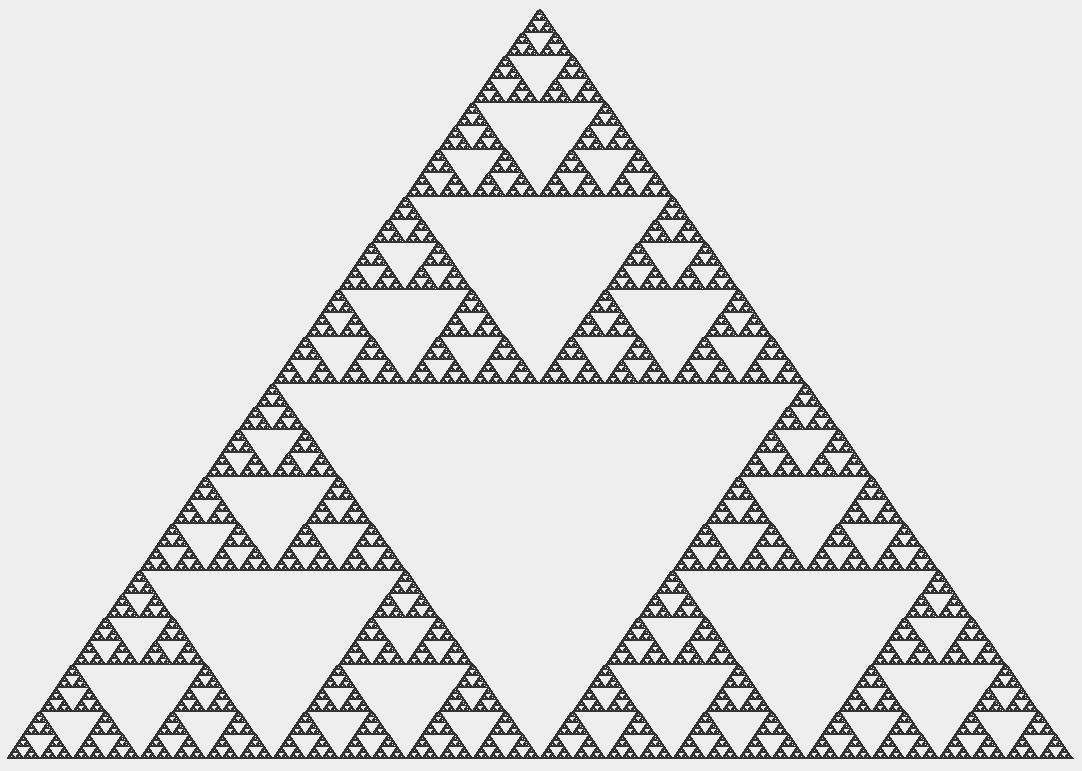
\includegraphics[width=0.8\textwidth]{srp.PNG}
